%%% Local Variables:
%%% mode: latex; mode: flyspell
%%% TeX-master: "."
%%% End:

\section { Fits }

To fit the endpoint energy for a given data spectrum, closure approximation spectra were convolved with a detector
response function using $\kmax$ values between 80 MeV and 100 MeV.
%% convolved spectra were generated for $\kmax$ values between 80 MeV and 100 MeV using both detector response functions.
Each convolved spectrum was scaled to minimize the $\chi^2$ and then the negative log likelihood ($\mathcal{L}$).
%%, where the latter is able to take into account empty bins in the data while the former cannot. 
For the $\mathcal{L}$ minimization, the convolved spectrum value in each bin was taken as the mean 
of a Poisson distribution in this bin.
%% The scale factors to minimize the $\chi^2$ and $\mathcal{L}$ fits were derived by:

%% $$f_{Poisson}(N;x_i) = \frac{x_i^N e^{-x_i}}{N!}$$
%% $$\chi^2 = \sum^N_{i=1} (\frac{A*x_i - y_i}{\sigma_i})^2; \mathcal{L} = -\sum^N_{i=1}log(f_{Poisson}(y_i;A*x_i))$$
%% $$\frac{\partial \mathcal{L}}{\partial A} = 0 \rightarrow A_{\mathcal{L}} = \frac{\sum^N_{i=1} y_i}{\sum^N_{i=1} x_i} $$
%% $$\frac{\partial \chi^2}{\partial A} = 0 \rightarrow A_{\chi^2} = \frac{\sum^N_{i=1} \frac{x_i*y_i}{\sigma_i^2}}{\sum^N_{i=1} \frac{x_i^2}{\sigma_i^2}} $$

%% \noindent
%% where $x_i$ is the predicted value corresponding to data $y_i$ for a given endpoint value.

The distribution of $\chi^2$ and $\mathcal{L}$ values as a function of the endpoint energy were each fit to a parabola near 
their minima to find the best fit endpoint energy. The estimated uncertainty on the endpoint energy is then
defined by $\Delta \chi^2 = 1$ and $\Delta \mathcal{L} = \frac{1}{2}$. This was done using both published detector response
functions, an example fit using the 1992 detector response function
and the 1992 aluminum data is shown in Figure \ref{fig:1992AlFits}. 

The fit $\kmax$ values for all 
datasets and both detector response functions are shown in Figures \ref{fig:ChiSq} and \ref{fig:NLL}, and the $\chi^2$/DOF
distributions are shown in Figure \ref{fig:ChiSqOfFits}. 
%% Should we include the Chi^2 for the NLL fit? Should we define what this means?
%% See Fitter::DoBinnedLikelihoodFit(bool extended) where defines the chi^2 using the data
%% and likelihood function. So straightforward chi^2 with errors from spectrum?
The $\chi^2$/DOF peaks around 1 for the 1998 detector response 
function and does not have the expected shape for the 1992 detector response function. Figure \ref{fig:compareFits}
shows the difference between the $\mathcal{L}$ and the $\chi^2$ fits for both detector response functions.
Figure \ref{fig:ToyFitErrs} shows the errors in fitting toy data generated with
an endpoint energy of 90 MeV. The toy fits shows that the expected difference between the $\chi^2$ and $\mathcal{L}$ fits 
is around 0.5 MeV. The difference between the two fits for the data is around 1 MeV for the fits using the 1998 detector 
response function and around 3 MeV when using the 1992 detector response function, consistent with the 1992 detector response 
not describing the data well. 

A possible source of the discrepancy between the $\chi^2$ and $\mathcal{L}$ fits is a small background 
in the high energy region of the data, which would skew the $\mathcal{L}$ fit $\kmax$ values up due to the high weight they would hold for deviating
from the convolved spectra. In the data spectrum shown in Figure \ref{fig:1992AlFits} there appears to be 3 high energy events above 95 MeV
not consistent with the expected spectrum. One could account for a background like this by removing the top 0.5\% of the data and refitting the remaining
data. Figure \ref{fig:compareFitsTopCut} shows the difference between the fits after this cut on the data, where the 
mean difference is now around 2 MeV for the 1992 detector response function, which is still inconsistent with expectations from
the toy MC studies, and around 0.5 MeV for the 1998 detector response function, which is consistent with the toy MC studies.
The toy MC studies suggest that the $\mathcal{L}$ fit $\kmax$ values are closer to the true energy due to a bias of around 0.5 MeV 
in the $\chi^2$ fits.

%%  where the $\mathcal{L}$ fit $\kmax$ values are consistently higher which is consistent
%% with $\mathcal{L}$ being more sensitive to bins with low entries.

%% The published data was fit using both of the published response functions.
%% The method to fit the data was to minimize the $\chi^2$ value for many values
%% of kMax, and then fit a parabola to the $\chi^2$ distribution, 
%% $\chi^2_{Min} + \frac{(k-kMax)^2}{\sigma^2}$. The uncertainty on the fit kMax
%% is then the inverse square root of the coefficient. This was also done using
%% a negative log likelihood ($\mathcal{L}$) minimization strategy, where the variance is half of
%% the inverse of the leading coefficient. 
%% The latter is able to take into account empty
%% bins in the data while the former cannot. The $\kmax$ values for each target Z 
%% are shown in Figure \ref{fig:ChiSq} and \ref{fig:NLL} using $\chi^2$ and $\mathcal{L}$ minimization
%% respectively, and the $\chi^2$/DOF is shown in Figure \ref{fig:ChiSqOfFits}. The $\mathcal{L}$
%% fitting method includes empty bins, which are ignored by the $\chi^2$ fitting method,
%% and has a greater cost for deviating from bins with small entry numbers. This results
%% in the $\mathcal{L}$ fit $\kmax$ values being consistently higher, as is shown in Figure \ref{fig:compareFits}.

\begin{figure}[h]
  \centering
  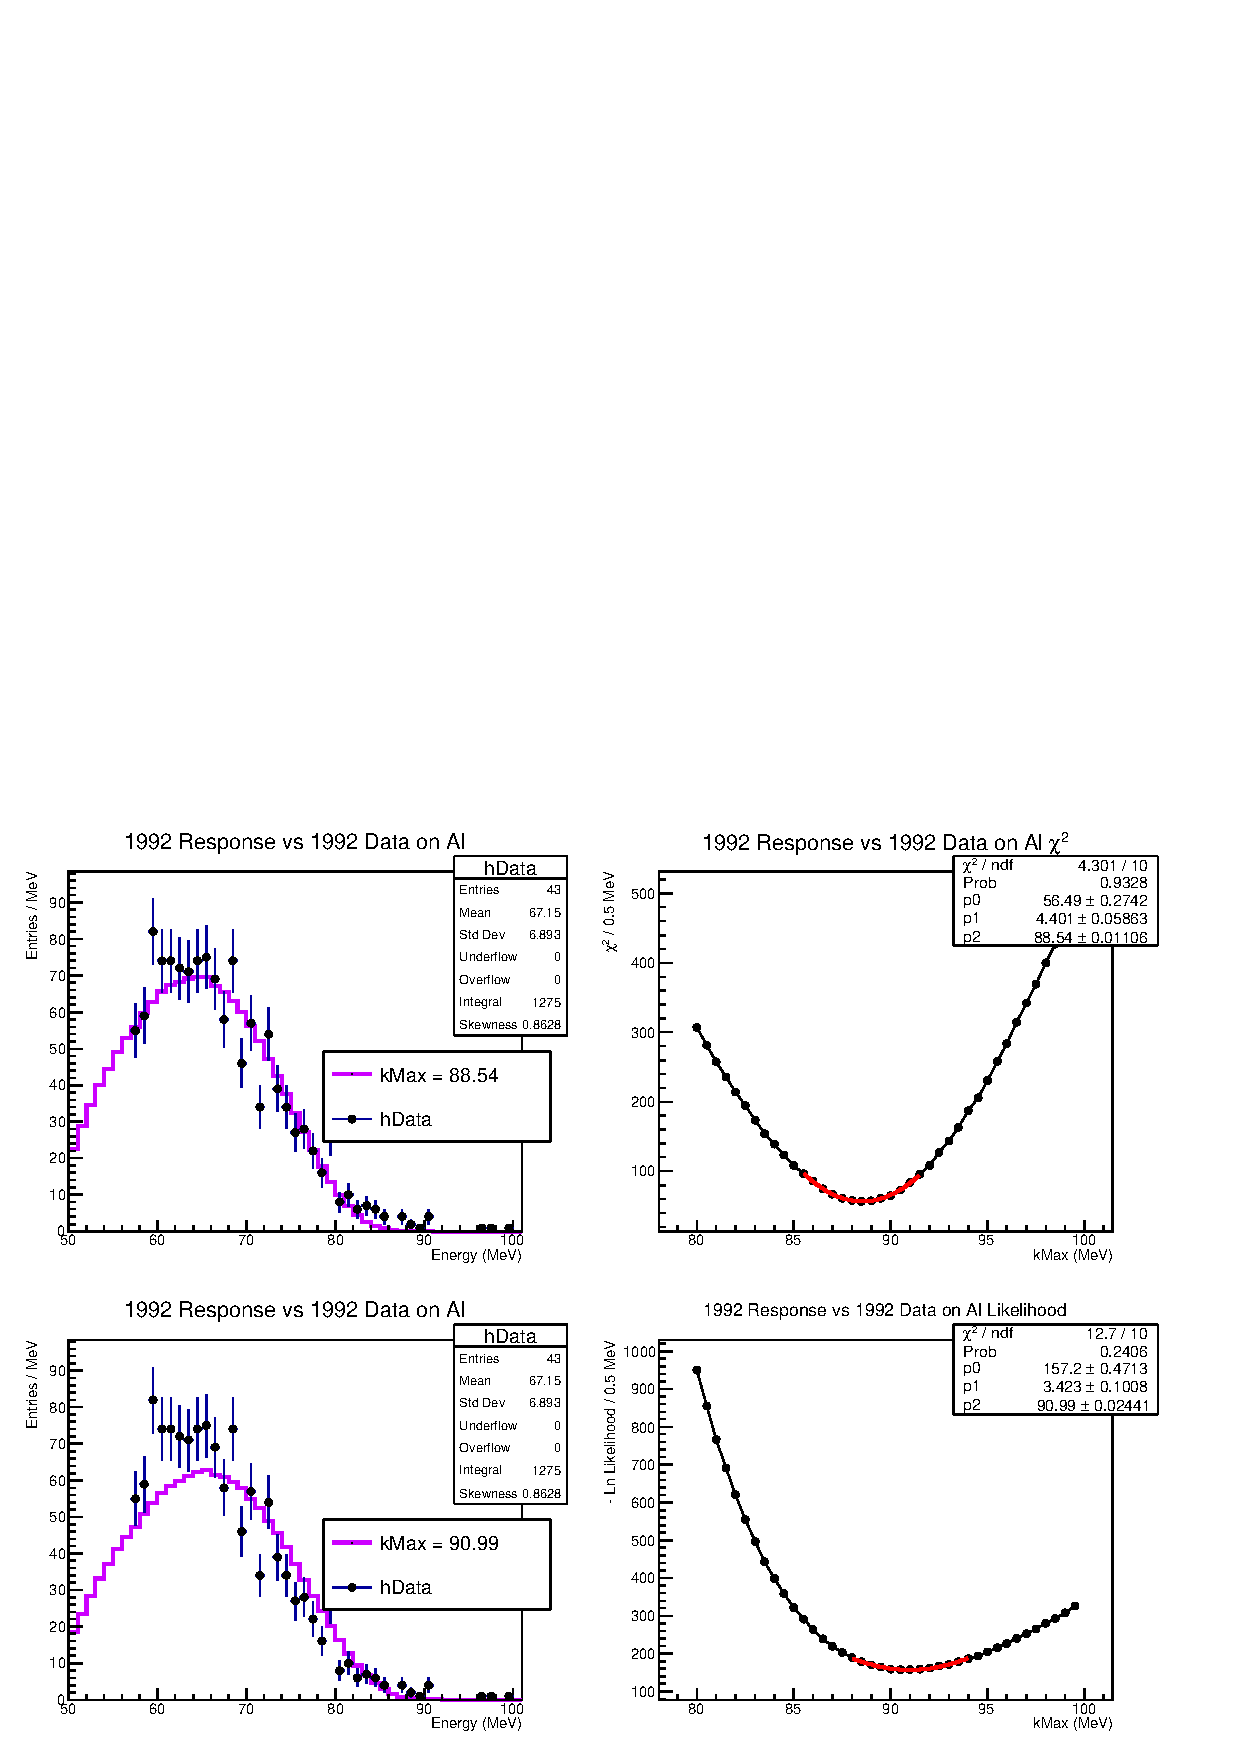
\includegraphics[width=0.8\linewidth]{figures/png/1992_resp_1992_Al_data_allPlots_singleK.png}
  \caption{The left figures show the best fit convolved closure approximation spectrum. The right figures
  show the parabolic fit to find the best fit endpoint energy. The top figures use $\chi ^2$ 
  minimization while the bottom figures use $\mathcal{L}$ minimization.}
  \label{fig:1992AlFits}
\end{figure}


\begin{figure}[h]
  \centering
  \subfloat[ $\chi^2$ Minimization Fit \label{fig:ChiSq}]{%
  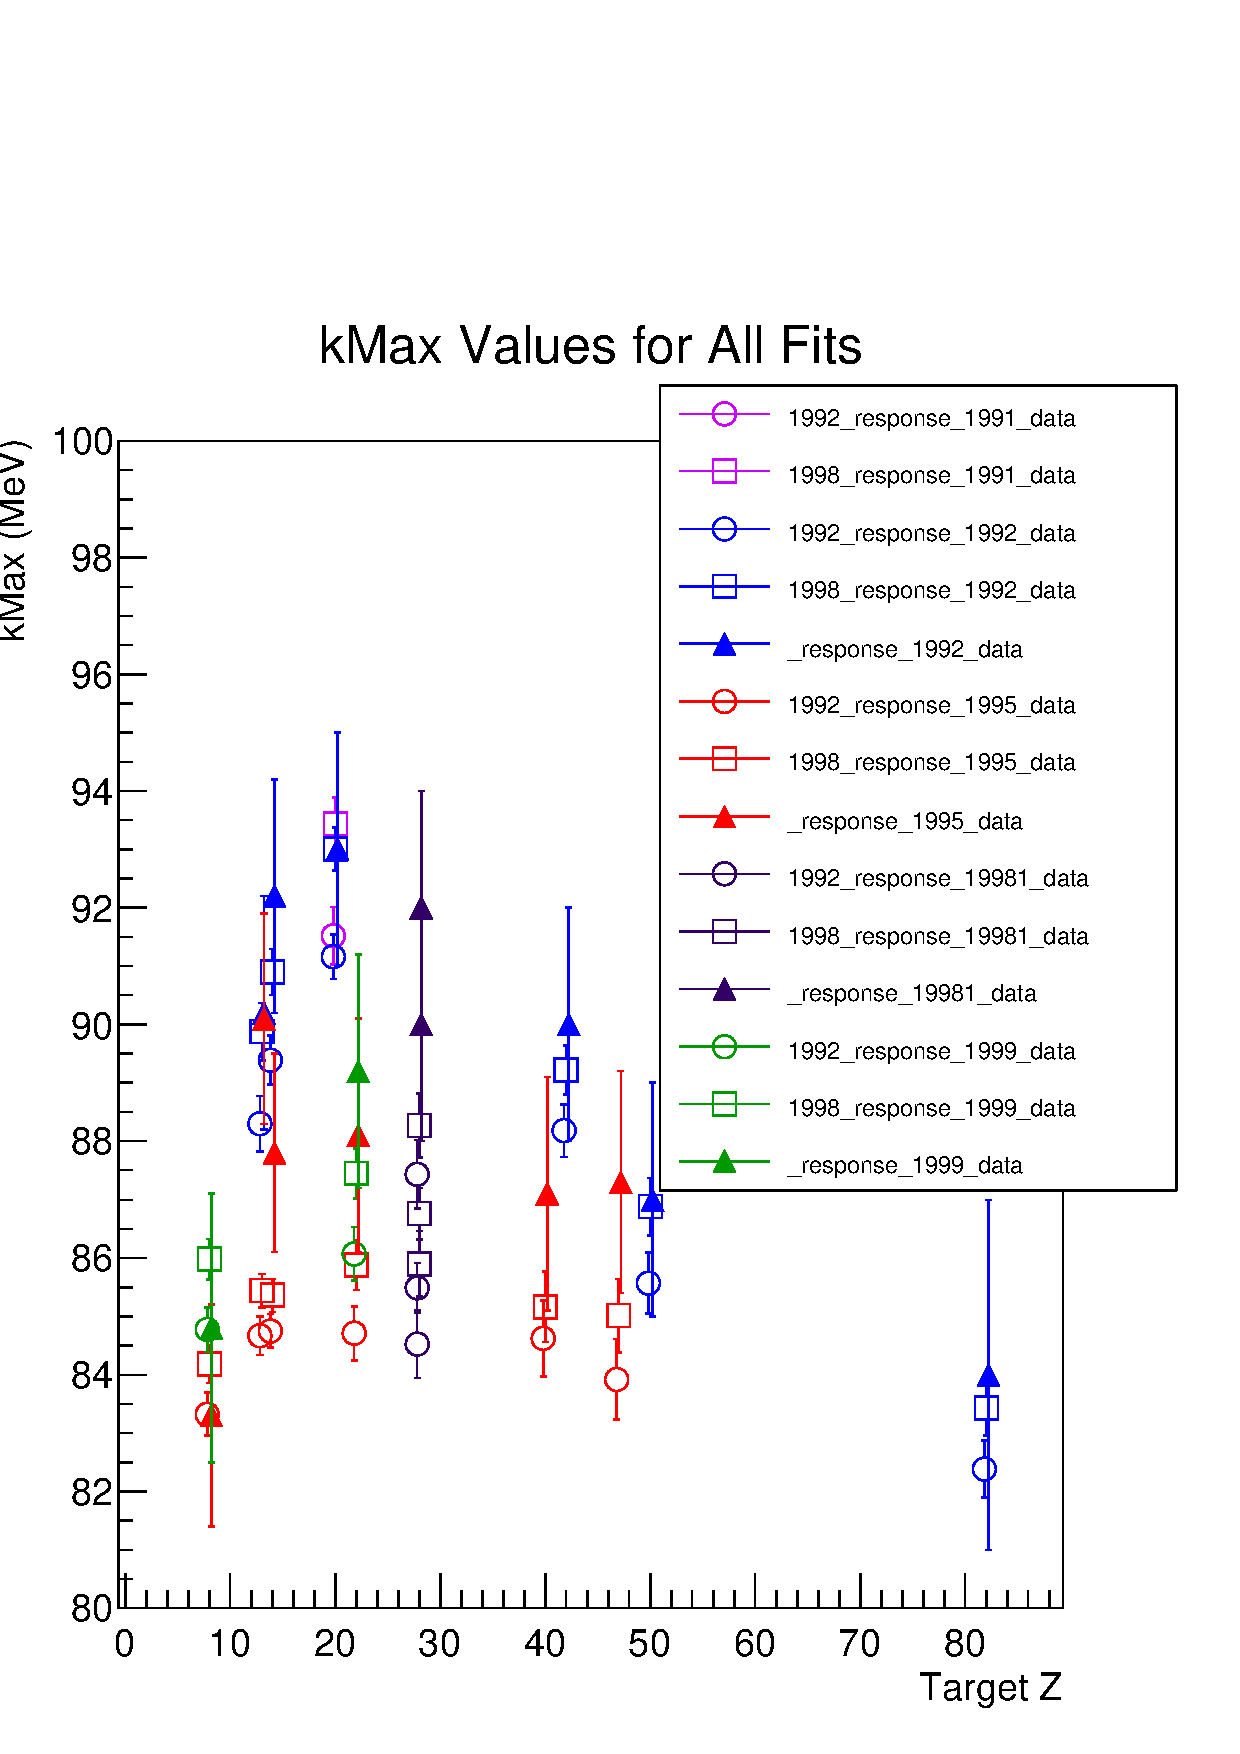
\includegraphics[width=0.48\linewidth]{figures/png/all_kMaxesChiSq_vs_target_z.png}
  }
  \hfill
  \subfloat[$\mathcal{L}$ Minimization Fit  \label{fig:NLL}]{%
  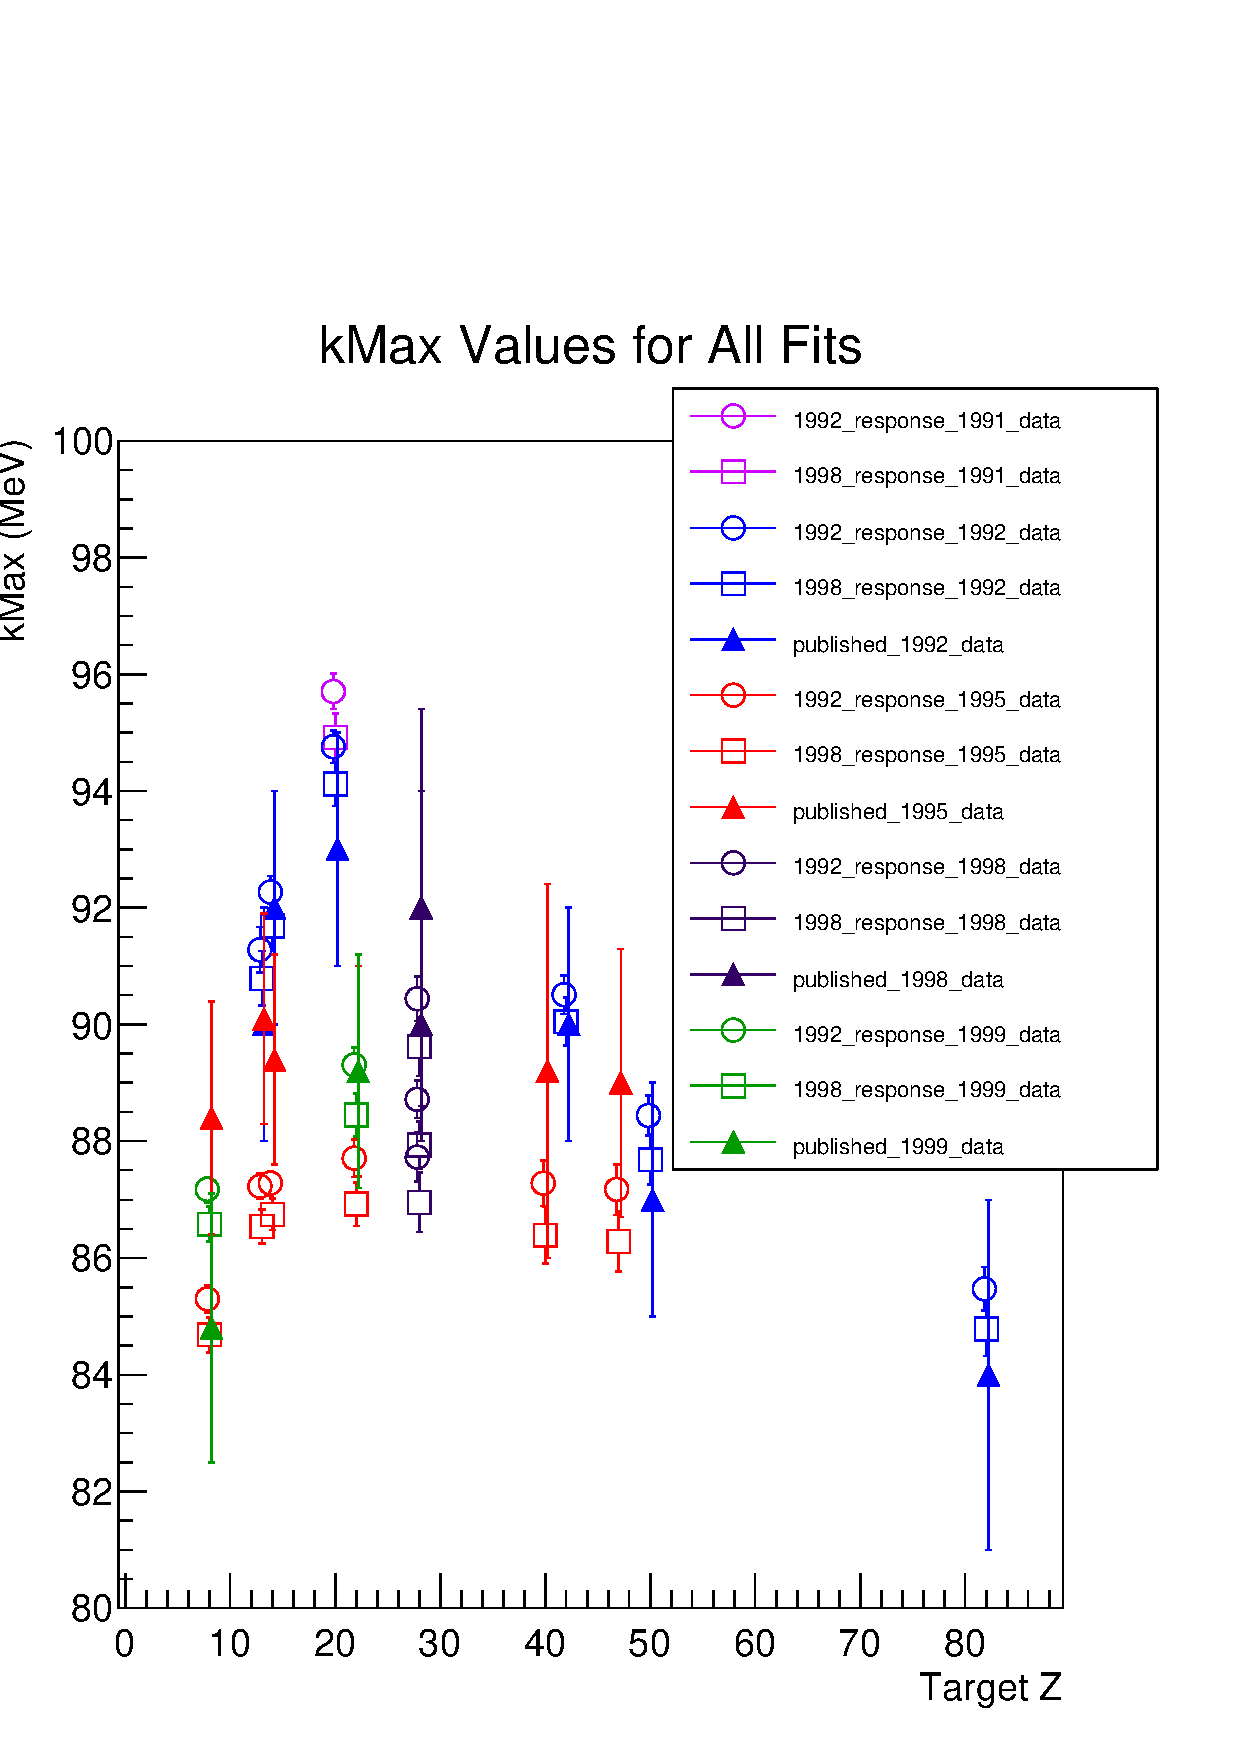
\includegraphics[width=0.48\linewidth]{figures/png/all_kMaxesNLL_vs_target_z.png}
  }
  \caption{Fit results vs target Z using (a) $\chi^2$ minimization and (b) $\mathcal{L}$ minimization.
    The 1992 detector response function data points (circles) are offset by -0.2 in z and the published data points (triangles)
    are offset by +0.2 in z.
  }
\end{figure}

%%%%%%%%%%%%%%%%%%%%%%%%%%%%%%%%%%%%%%%%%%%%%%%%%%%%%%%%%%%%%%%%%%%%%%%%%%%%%%%%%%%%%%%%%%%%%%%%%%%%%%
%% Should we include the chi square of the NLL fits, if we're not sure how they're defined in ROOT? %%
%%%%%%%%%%%%%%%%%%%%%%%%%%%%%%%%%%%%%%%%%%%%%%%%%%%%%%%%%%%%%%%%%%%%%%%%%%%%%%%%%%%%%%%%%%%%%%%%%%%%%%

\begin{figure}[h]
  \centering
  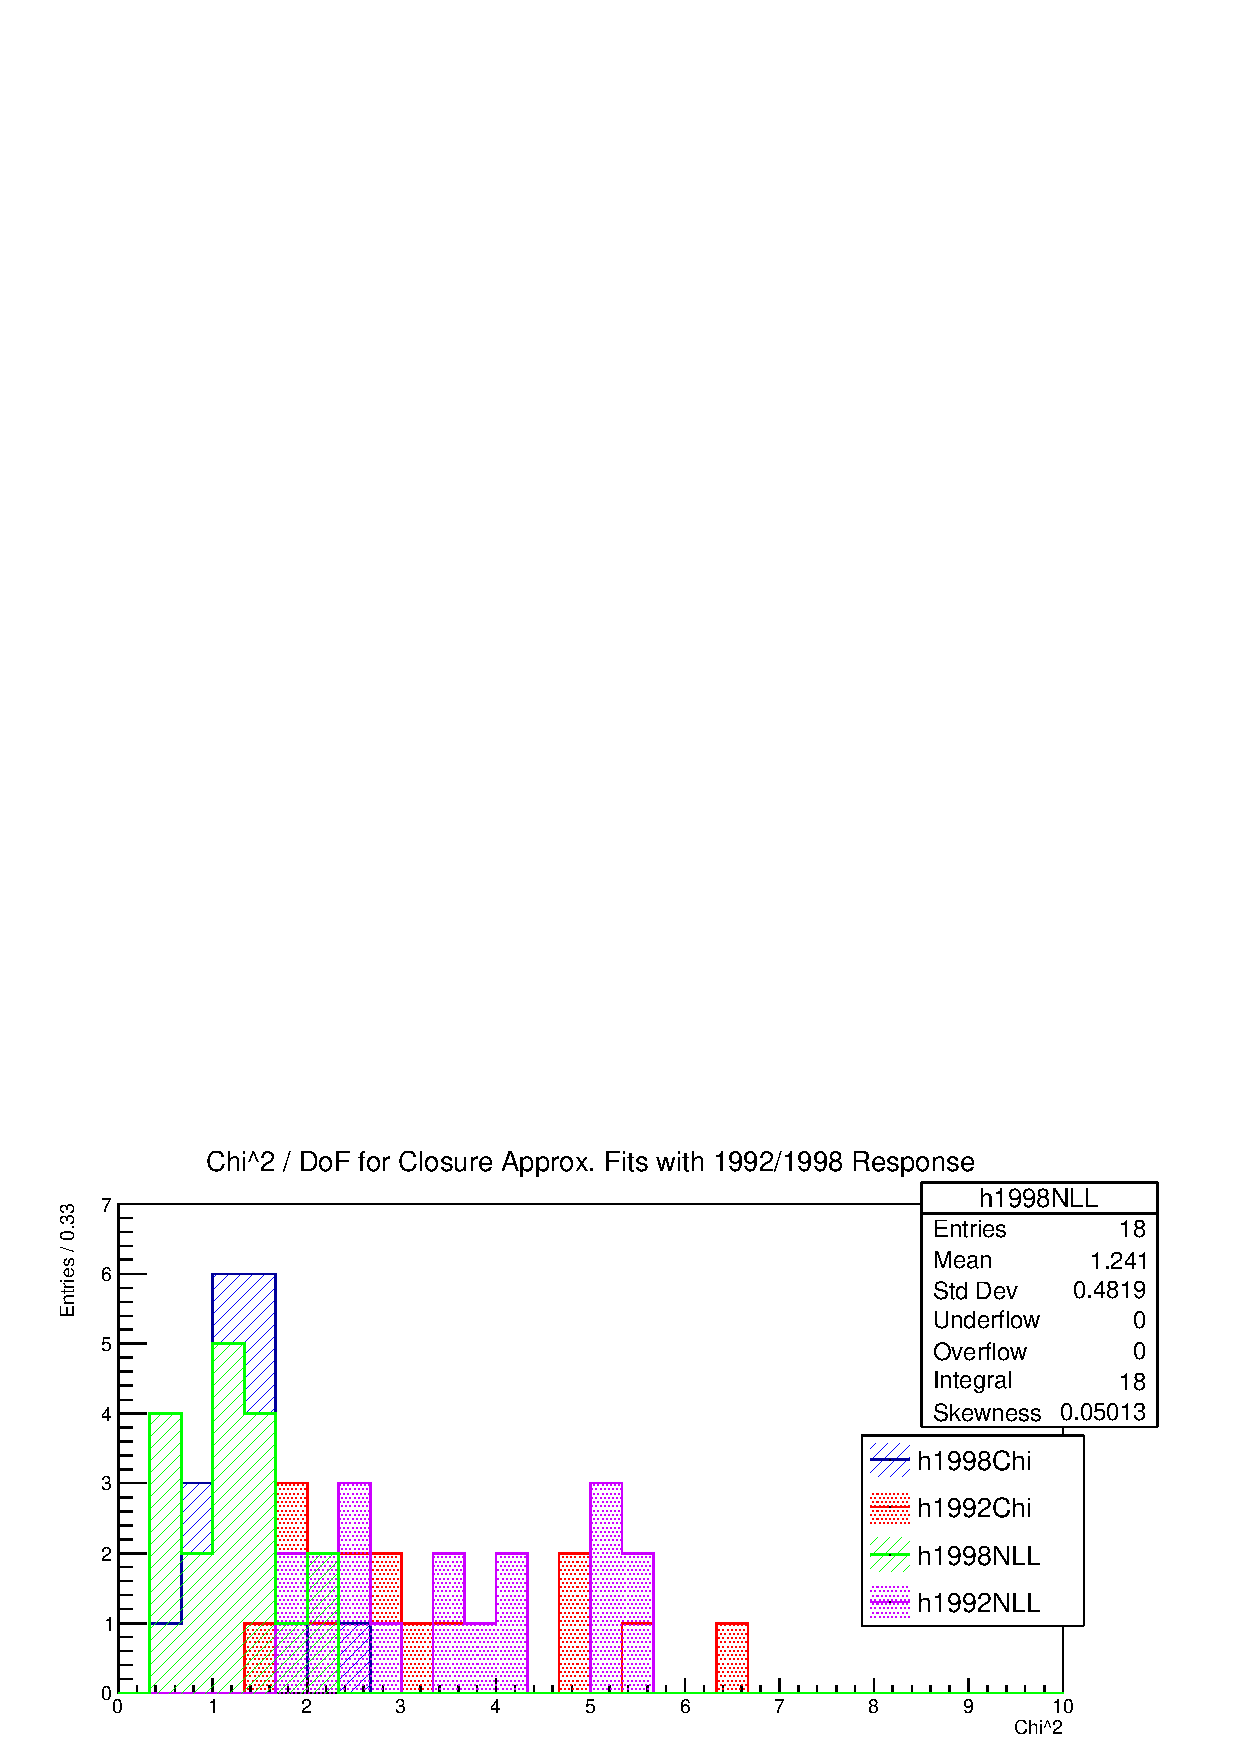
\includegraphics[width=0.8\linewidth]{figures/png/chiSq_of_fits.png}
  \caption{Fit $\chi^2$ values for both detector response functions and both fitting methods. }
  \label{fig:ChiSqOfFits}
\end{figure}


\begin{figure}[h]
  \centering
  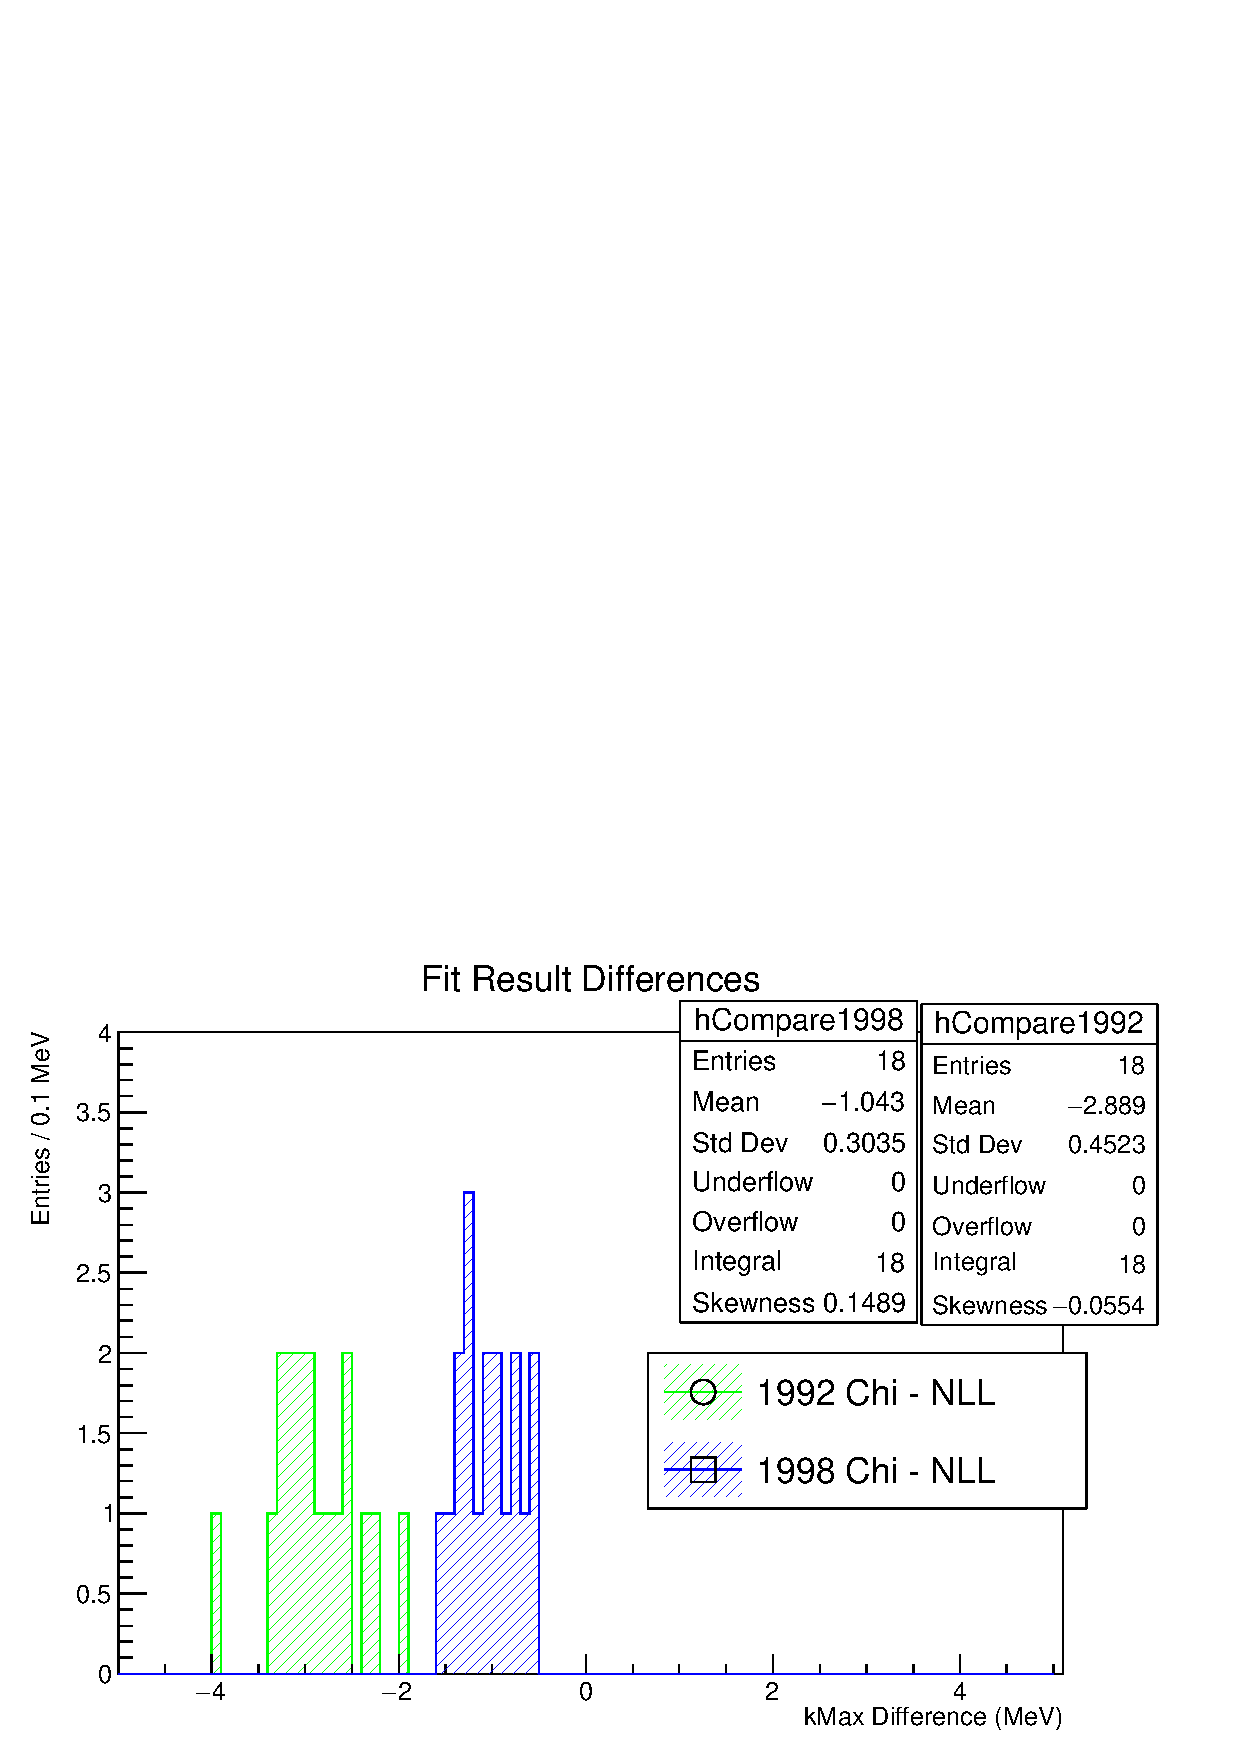
\includegraphics[width=0.8\linewidth]{figures/png/compare_fit_results_92_v_98_unrestrictedOnly.png}
  \caption{The difference between the $\kmax$ values found using $\chi^2$ and
    $\mathcal{L}$ minimization using the 1992 and 1998 detector response functions.}
  \label{fig:compareFits}
\end{figure}

\begin{figure}[h]
  \centering
  \subfloat[ 1992 detector response \label{fig:1992ToyErrs}]{%
  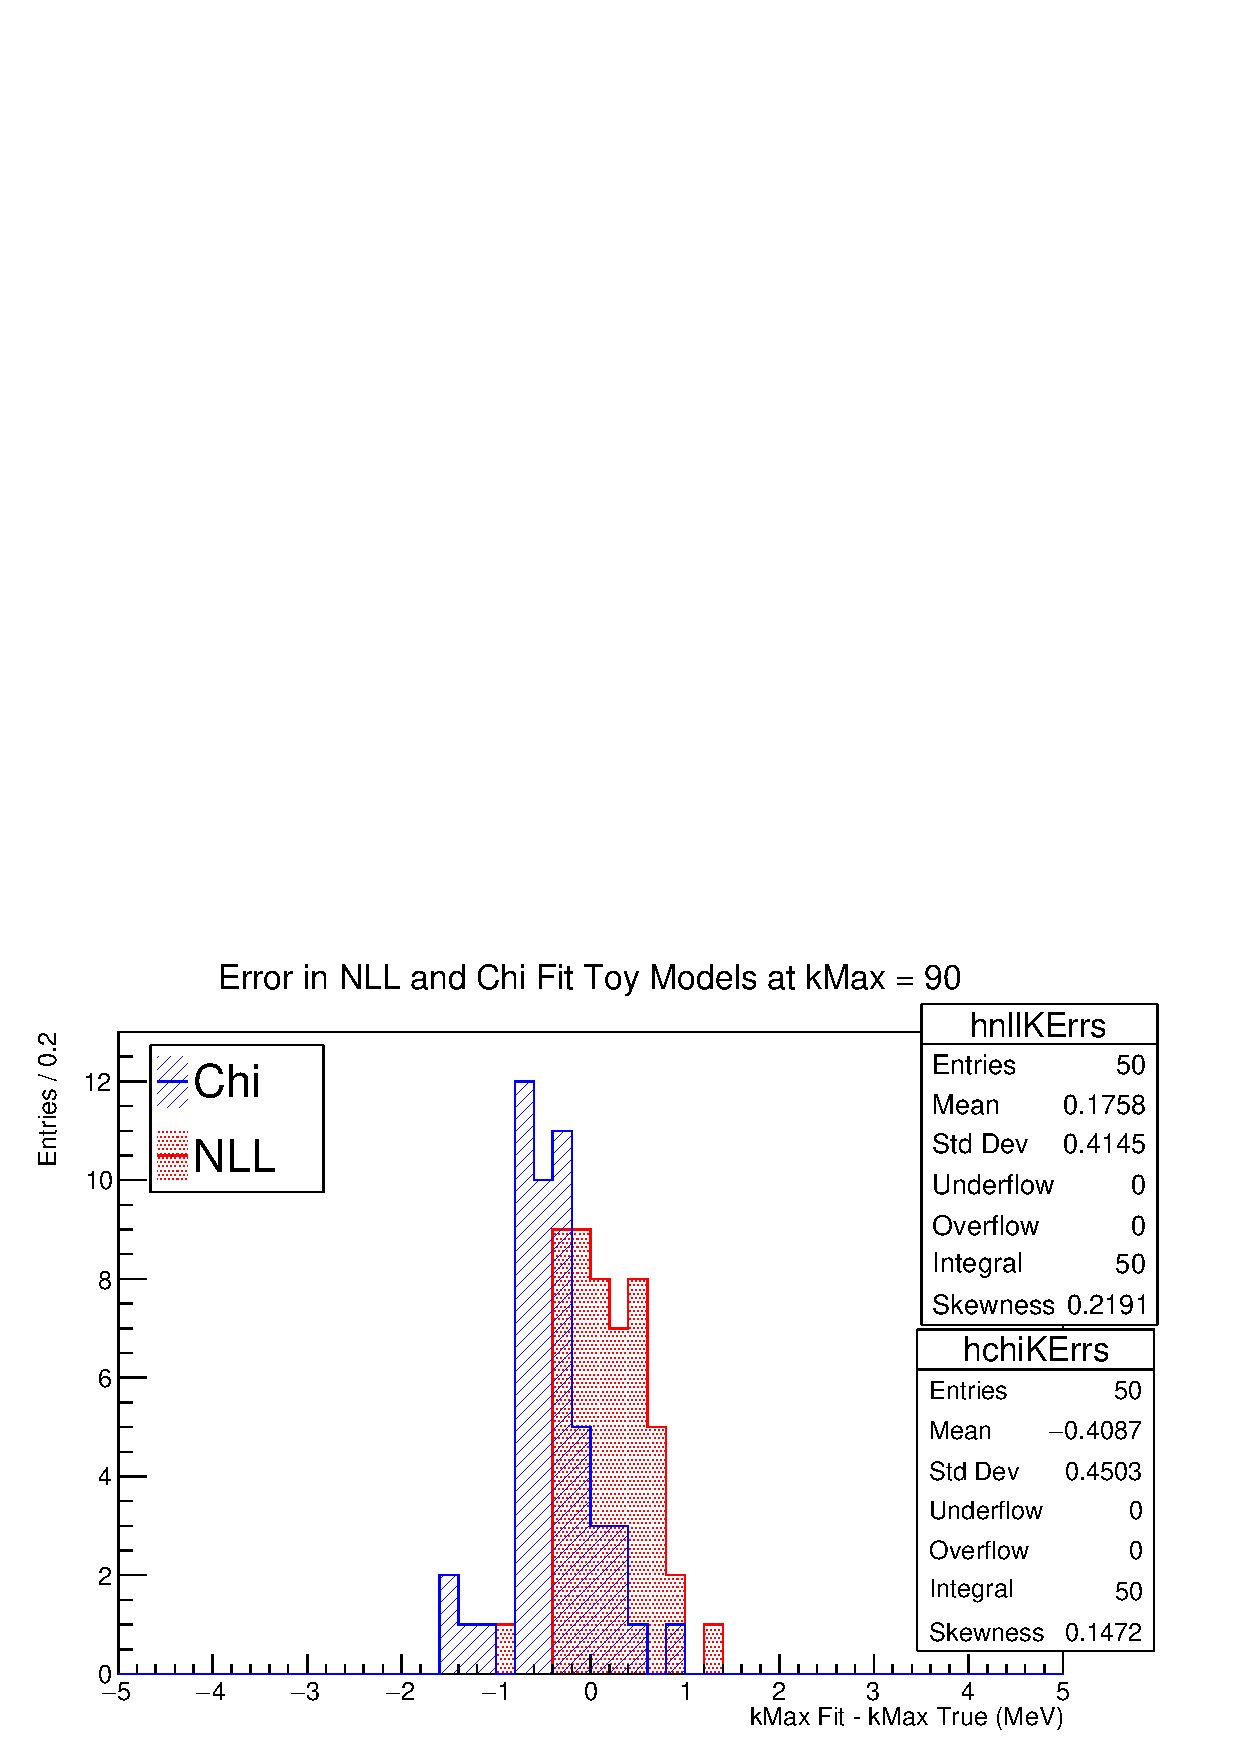
\includegraphics[width=0.48\linewidth]{figures/png/toy_kMax_errors_1992_response.png}
  }
  \hfill
  \subfloat[ 1998 detector response  \label{fig:1998ToyErrs}]{%
  \includegraphics[width=0.48\linewidth]{figures/png/toy_kMax_errors_1998_response.png}
  }
  \caption{Distributions for the fit bias $\Delta{K_{max}} = K_{max}^{fit}-K_{max}^{true}$ for 50 toy %
    data sets using the (a) 1992 or (b) 1998 detector response function.
    The toy data sets are generated from a convolution with an endpoint energy of 90 MeV
    and generated with 1275 data points.
  }
  \label{fig:ToyFitErrs}
\end{figure}

\begin{figure}[h]
  \centering
  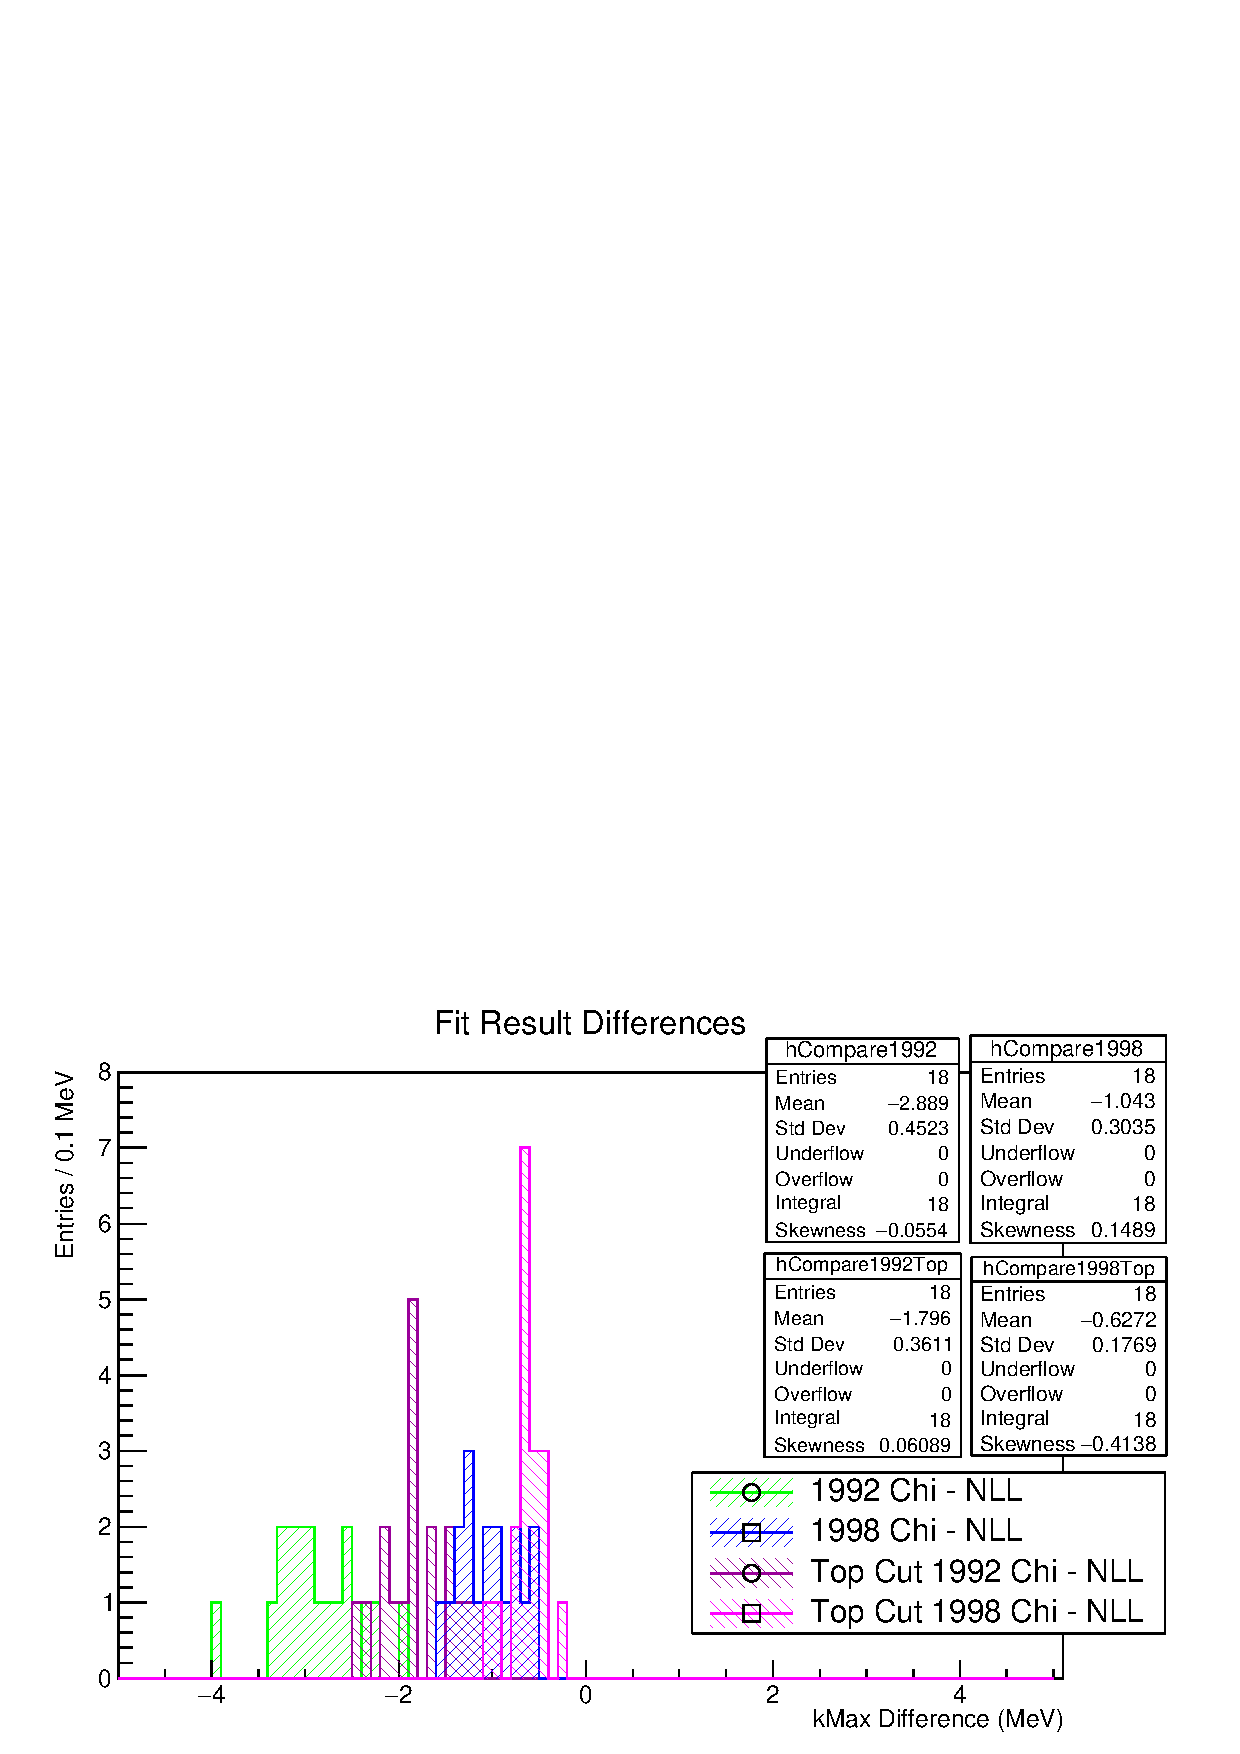
\includegraphics[width=0.7\linewidth]{figures/png/compare_fit_results_92_v_98_with_topCut.png}
  \caption{The difference between the $\kmax$ values found using $\chi^2$ and
    $\mathcal{L}$ minimization with and without excluding the top 0.5\% of the data
    using the 1992 and 1998 detector response functions.}
  \label{fig:compareFitsTopCut}
\end{figure}


%% \begin{figure}[h]
%%   \centering
%%   \subfloat[ 1992 detector response \label{fig:1992ToyZs}]{%
%%   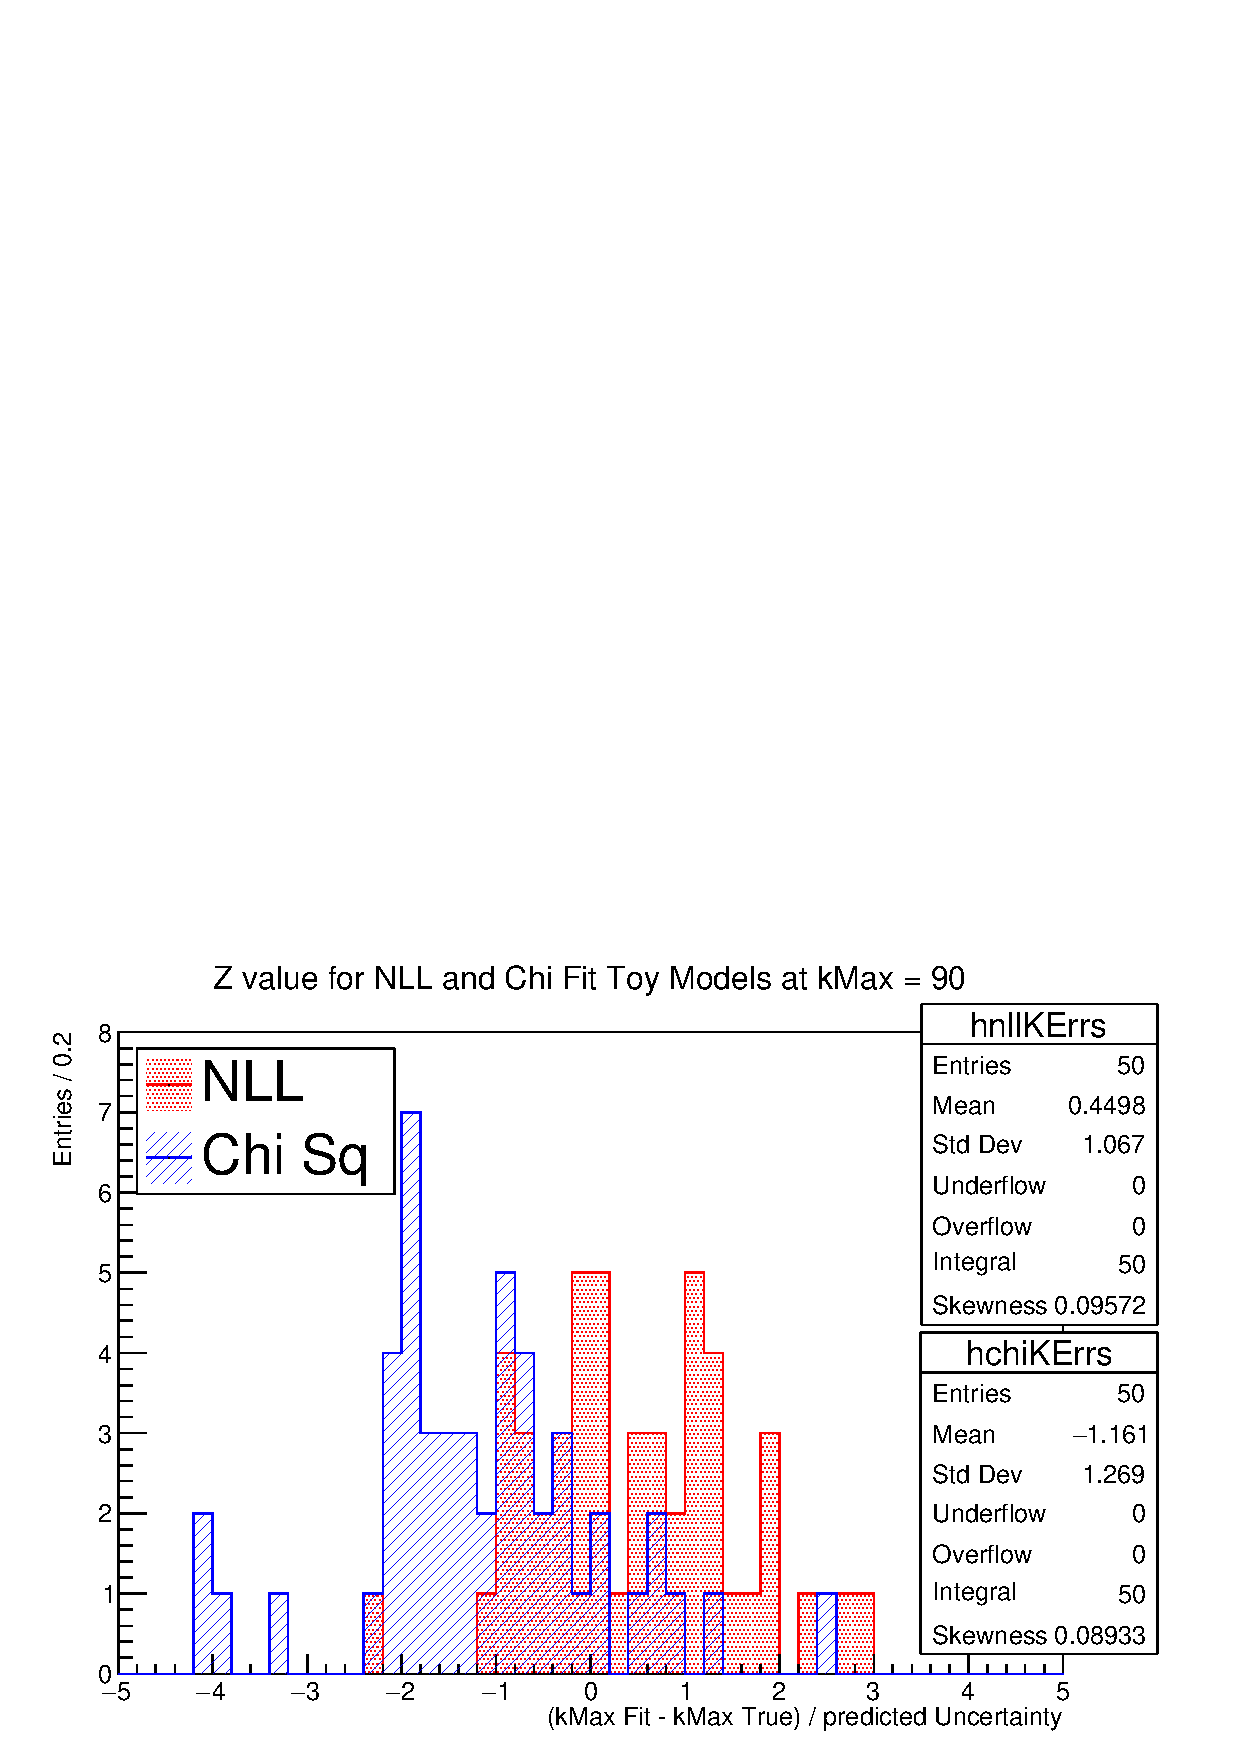
\includegraphics[width=0.48\linewidth]{figures/png/toy_kMax_z_values_1992_response.png}
%%   }
%%   \hfill
%%   \subfloat[ 1998 detector response  \label{fig:1998ToyZs}]{%
%%   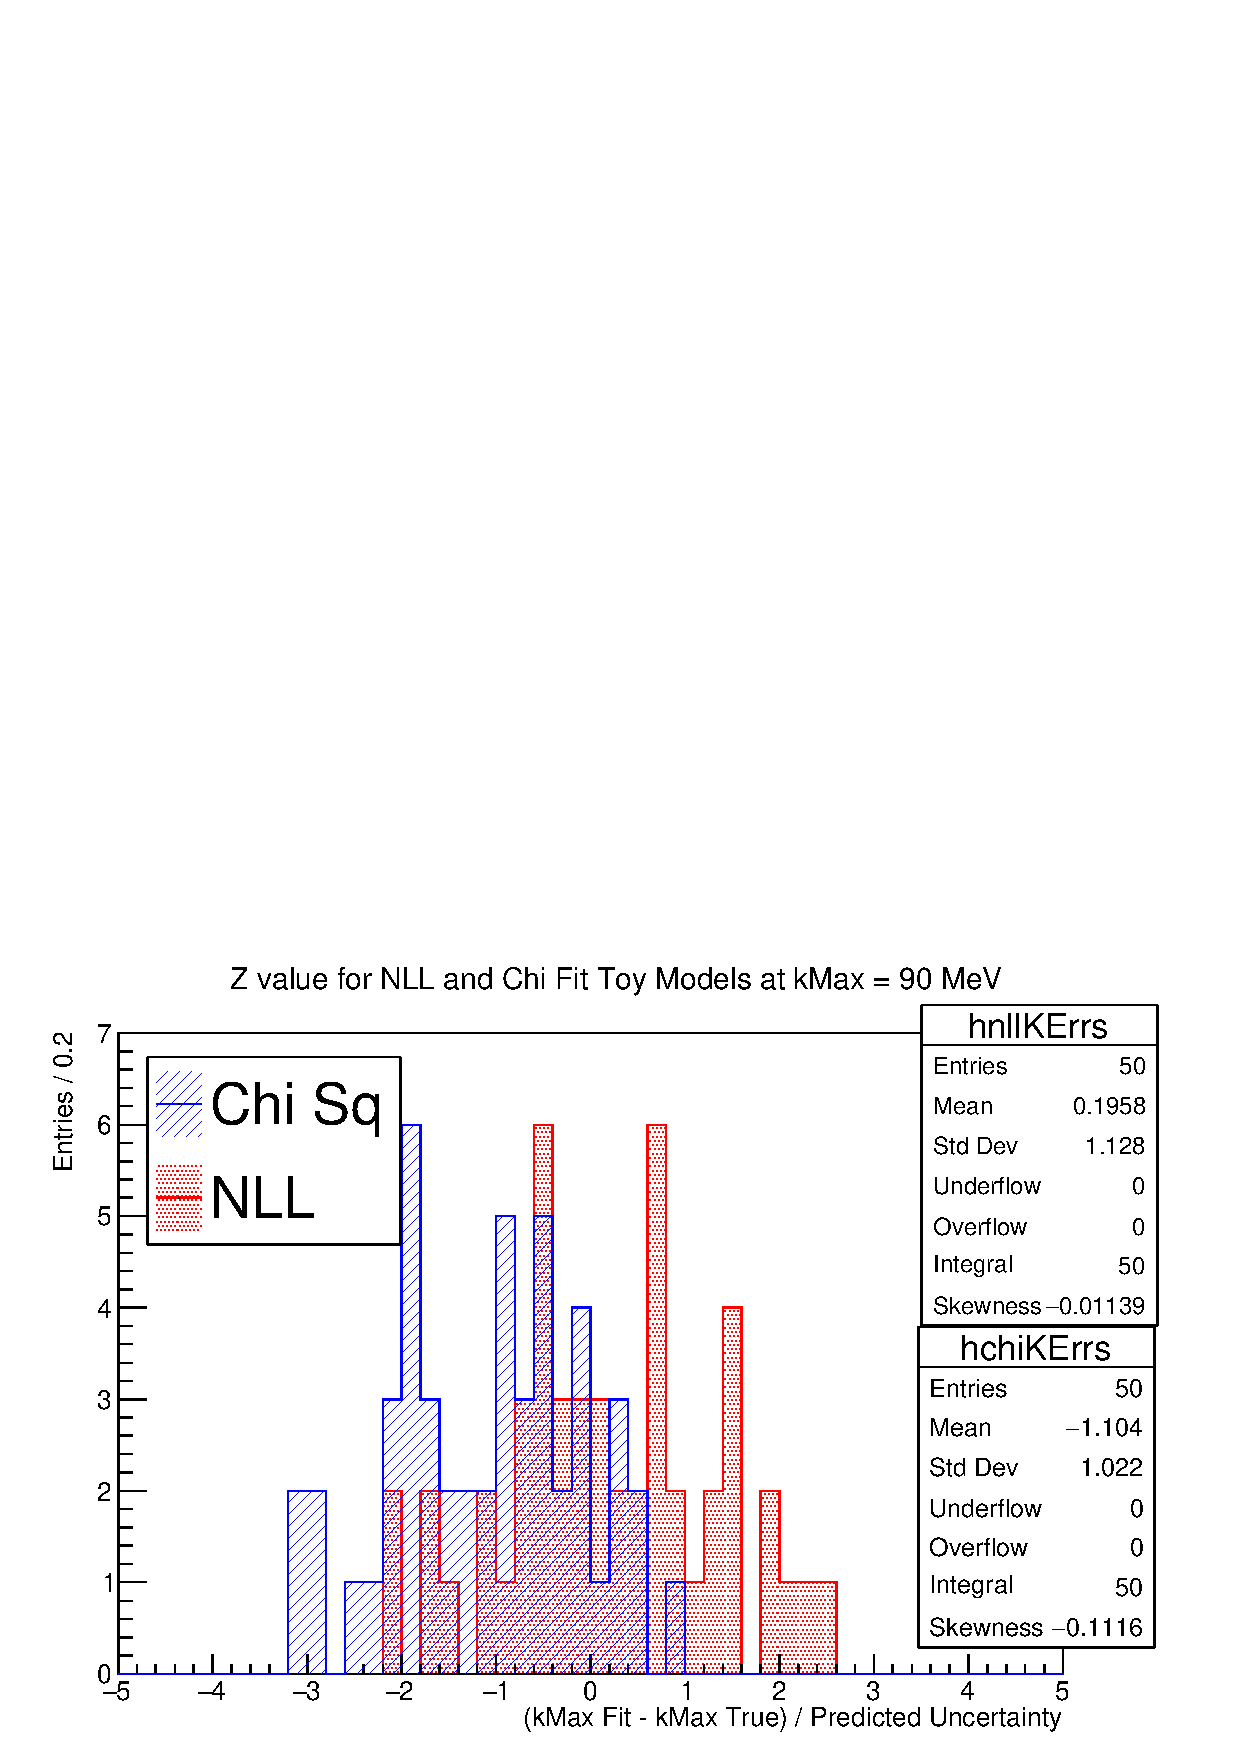
\includegraphics[width=0.48\linewidth]{figures/png/toy_kMax_z_values_1998_response.png}
%%   }
%%   \caption{Fit results z values for 50 toy data sets using the (a) 1992 or (b) 1998 detector response function.
%%     The toy data sets are generated from a convolution with an endpoint energy of 90 MeV and generated
%%     with 1275 data points. The z value for a fit is the fit endpoint value minus the true value, divided
%%     by the fit estimated uncertainty. 
%%   }
%%   \label{fig:ToyFitZs}
%% \end{figure}



